\documentclass[landscape,debug,paperwidth=1510mm, paperheight=955mm,]{xebaposter}

\usepackage{url}
\usepackage{amsmath}
\usepackage{amssymb}
%\usepackage{relsize}
%\usepackage{graphicx}
\usepackage{multicol}
\usepackage{xecolor}
%\usepackage[verbose]{wrapfig}
\graphicspath{{images/}}
\usepackage[inline]{enumitem}% for making inline list.
\setlist{noitemsep}% Save space in lists.
\usepackage{listings}
\usepackage{fancyvrb}
\usepackage{atbegshi}
\usepackage[Kashida=off]{xepersian}
\settextfont{Yas}
\setdigitfont{Yas}


\lstset{% general command to set parameter(s)
    language=[LaTeX]tex,
    basicstyle=\setLTR\ttfamily,
    gobble=0,
    breaklines=true,
}
 %%%%%%%%%%%%%%%%%%%%%%%%%%%%%%%%%%%%%%%%%%%%%%%%%%%%%%%%%%%%%%%%%%%%%%%%%%%%%%%%
 %%%% Some math symbols used in the text
 %%%%%%%%%%%%%%%%%%%%%%%%%%%%%%%%%%%%%%%%%%%%%%%%%%%%%%%%%%%%%%%%%%%%%%%%%%%%%%%%
 % Format
% \newcommand{\RotUP}[1]{\begin{sideways}#1\end{sideways}}


 %%%%%%%%%%%%%%%%%%%%%%%%%%%%%%%%%%%%%%%%%%%%%%%%%%%%%%%%%%%%%%%%%%%%%%%%%%%%%%%%
 % Multicol Settings
 %%%%%%%%%%%%%%%%%%%%%%%%%%%%%%%%%%%%%%%%%%%%%%%%%%%%%%%%%%%%%%%%%%%%%%%%%%%%%%%%
% \setlength{\columnsep}{0.7em}
% \setlength{\columnseprule}{0mm}

%%% Setting User Defined Background %%%%%%%%%%%%%%%%%%%%%%%%%%%%%%%%%%%%%%%%%%%%%%
%if you want to use your preferred background, you should set background=user in poster settings.
\background{
  \begin{tikzpicture}[remember picture,overlay,opacity=.3]%
    \fill [yellow!80!gray] {(current page.south east) rectangle (current page.north west)};%
%	\draw (current page.south west)+(12em,0em) node[anchor=south west,opacity=.3]
%	{
\includegraphics[width=.2\textwidth]{logo}};
  \end{tikzpicture}%
}
%% Begin of Document
%%%%%%%%%%%%%%%%%%%%%%%%%%%%%%%%%%%%%%%%%%%%%%%%%%%%%%%%%%%%%%%%%%%%%%%%%%%%%
\begin{document}

%\newcommand\back{
%    \makeatletter
%%  \setLTR\begin{bidi@tikzpicture}[remember picture,overlay,opacity=.3]%
%  \begin{tikzpicture}[remember picture,overlay,opacity=.3]%
%    \setLTR\fill [green!20!yellow] {(current page.south east) rectangle (current page.north west)};%
%	\draw (current page.north west)+(-2em,2em) node[anchor=north west,opacity=.3]
%	{
\includegraphics[width=1.1\textwidth]{logo}};
%%  \end{bidi@tikzpicture}%
%  \end{tikzpicture}%
%  \makeatother
%}
%\AtBeginShipoutInit
%\AtBeginShipout{\AtBeginShipoutAddToBox{\back}}
%%%%%%%%%%%%%%%%%%%%%%%%%%%%%%%%%%%%%%%%%%%%%%%%%%%%%%%%%%%%%%%%%%%%%%%%%%%%%
%% Here starts the poster
%%---------------------------------------------------------------------------
%% Format it to your taste with the options
%%%%%%%%%%%%%%%%%%%%%%%%%%%%%%%%%%%%%%%%%%%%%%%%%%%%%%%%%%%%%%%%%%%%%%%%%%%%%
      \definecolor{silver}{cmyk}{0,0,0,0.3}
      \definecolor{yellow}{cmyk}{0,0,0.9,0.0}
      \definecolor{reddishyellow}{cmyk}{0,0.22,1.0,0.0}
      \definecolor{black}{cmyk}{0,0,0.0,1.0}
      \definecolor{darkYellow}{cmyk}{0,0,1.0,0.5}
      \definecolor{darkSilver}{cmyk}{0,0,0,0.1}

      \definecolor{lightyellow}{cmyk}{0,0,0.3,0.0}
      \definecolor{lighteryellow}{cmyk}{0,0,0.1,0.0}
      \definecolor{lighteryellow}{cmyk}{0,0,0.1,0.0}
      \definecolor{lightestyellow}{cmyk}{0,0,0.05,0.0}

      \begin{poster}%
      % Poster Options
      {
      eyecatcher=true,
      % Color style
      bgColorOne=lighteryellow,%green!40!yellow!30,%lighteryellow,
      bgColorTwo=yellow,
      borderColor=reddishyellow,
      headerColorOne=yellow,
      headerColorTwo=reddishyellow,
      headerFontColor=cyan,
      boxColorOne=lightyellow,
      boxColorTwo=lighteryellow,
      % Format of textbox
      textborder=rounded,
      % Format of text header
      headerborder=closed,
%      headerheight=.07\textheight,
      headershape=roundedleft,
      headershade=plain,
%      headerfont=\Large, %Sans Serif
      boxshade=plain,
      background=user,
      linewidth=2pt,
      grid=false, % show a grid mesh on poster, it's useful for debugging.
      columns=5,
      }
 % Eye Catcher
 {
      
\includegraphics[height=0.05\textheight]{logo}
 }
 % Title
 {طراحی پوستری زیبا و در خور با کمک کلاس \lr{xebaposter}
}
 % Authors
 {\large \lr{Brian Amberg}, \lr{Reinhold Kainhofer}, سیّدمحمّدجواد رضویان
 \\%[1em]
 {\normalsize\texttt{\lr{javadr@parsilatex.com, reinhold@kainhofer.com, baposter@brian-amberg.de}}
 \\
نسخه $2.53$، $18$ خرداد $1401$، $8$ ژوئن $2022$
 }}
 % University logo
 {
    
\includegraphics[height=0.05\textheight]{logo}
 }
% \end{poster}
% \end{document}
%%%%%%%%%%%%%%%%%%%%%%%%%%%%%%%%%%%%%%%%%%%%%%%%%%%%%%%%%%%%%%%%%%%%%%%%%%%%%%
%%% Now define the boxes that make up the poster
%%%---------------------------------------------------------------------------
%%% Each box has a name and can be placed absolutely or relatively.
%%% The only inconvenience is that you can only specify a relative position
%%% towards an already declared box. So if you have a box attached to the
%%% bottom, one to the top and a third one which should be inbetween, you
%%% have to specify the top and bottom boxes before you specify the middle
%%% box.
%%%%%%%%%%%%%%%%%%%%%%%%%%%%%%%%%%%%%%%%%%%%%%%%%%%%%%%%%%%%%%%%%%%%%%%%%%%%%%

 %%%%%%%%%%%%%%%%%%%%%%%%%%%%%%%%%%%%%%%%%%%%%%%%%%%%%%%%%%%%%%%%%%%%%%%%%%%%%%
\begin{posterbox}[name=introduction,column=0,row=0,headershape=smallrounded,
headershade=plain]%
{\textxecolor{red}{مقدمه}}
 %%%%%%%%%%%%%%%%%%%%%%%%%%%%%%%%%%%%%%%%%%%%%%%%%%%%%%%%%%%%%%%%%%%%%%%%%%%%%%
همانطوری که می‌دانید یکی از نیازهای جامعه علمی طراحی پوستر است زیرا که در برخی کنفرانس‌ها نویسنده مقاله تنها مجاز به ارائه پوستر
می‌گردد. در این راستا یک کلاس بسیار ساده به نام \texttt{a0poster} وجود دارد که در عین سادگی کار با آن، قابلیت‌های زیادی ندارد.
از طرفی دیگر کلاس‌های زیبایی برای تولید پوستر توسط افرادی دیگر طراحی شده است
از جمله \texttt{baposter}\footnote{\url{http://www.brian-amberg.de/uni/poster/}}،
\texttt{beamerposter} و \texttt{tikzposter}.
متاسفانه این کلاس‌ها با متون راست به چپ، خصوصاً فارسی کار نمی‌کنند لذا نیاز به کلاسی که بتوان با آن پوستر فارسی تولید کرد
ضروری می‌نمود. کلاس \texttt{xebaposter}% --بخوانید زیباپوستر--%
%از آنجایی که کلاس \texttt{baposter}
%بر پایهٔ \texttt{tikz} طراحی شده است و جناب آقای دکتر وفا خلیقی خالق
%بسته‌های \texttt{bidi} و \texttt{xepersian} امکان پشتیبانی از متون
%راست به چپ را در تصاویر تولیدی بسته \texttt{tikz} فراهم آورده‌اند پس بدین سبب به سراغ این کلاس رفته و با تغییراتی در آن،
%این کلاس را با متون راست به چپ خصوصا فارسی سازگار نموده و نام \texttt{xebaposter} را بر آن برگزیدیم%
%\footnote{نگارنده ابتدا نام \lr{baposterRL} را انتخاب کرده بود لکن با پیشنهاد دکتر محمود امین‌طوسی نام فعلی را برگزید.}
--بخوانید زیباپوستر--
 بر پایهٔ کلاس \texttt{baposter} با افزودن
امکاناتی بدین منظور بنا نهاده شده است.
%البته ناگفته نماند که پوسترهای تولیدی با بسته \texttt{beamerposter} زیبایی زاید الوصوفی دارند لکن به سبب اینکه بسته‌های
%بایدی و زی‌پرشین فعلا از بسته \texttt{beamer} پشتیبانی نمی‌کنند --آنهم به سبب وجود باگ‌هایی در موتور زی‌تک-- امکان
%فارسی‌سازی این بسته وجود نداشت پس بدین سبب تنها انتخابمان همان بسته اولیه \texttt{baposter} شد.
متاسفانه به سبب وجود باگ‌\footnote{گزارش شده در \url{http://qa.parsilatex.com/10715}
و \url{http://tex.stackexchange.com/questions/262877}} در موتور زی‌لاتک فعلاً ویژگی محوشدگی رنگ را
در حالت فارسی نخواهیم داشت.%
%\footnote{برای مشاهده
%نمونه‌هایی از این بسته‌ها می‌توانید به \url{http://www.latextemplates.com/cat/conference-posters} مراجعه نمایید.}
\end{posterbox}
%%%%%%%%%%%%%%%%%%%%%%%%%%%%%%%%%%%%%%%%%%%%%%%%%%%%%%%%%%%%%%%%%%%%%%%%%%%%%%
\begin{posterbox}[name=posterparts,column=0,span=1,below=introduction,textborder=roundedleft]
{\textxecolor{blue}{اجزاء تشکیل دهنده زیباپوستر}}
 %%%%%%%%%%%%%%%%%%%%%%%%%%%%%%%%%%%%%%%%%%%%%%%%%%%%%%%%%%%%%%%%%%%%%%%%%%%%%%
زیباپوستر صفحه پوستر را به دو بخش سرآمد  و محتوی تقسیم می‌کند. خود سرآمد نیز از سه بخش آی‌کچر، عنوان و لوگوی موسسه تشکیل
شده است که بهمین ترتیب نمایش داده می‌شود. بخش آی‌کچر اختیاری است و می‌توان با گزینه \texttt{eyecatcher} آن را فعال یا غیرفعال
نمود(\texttt{true,false}). در صورت عدم وجود آی‌کچر، عنوان و نام نویسنده‌(ها) راست چین خواهد شد و در صورت وجود آن به صورت
وسط‌چین در خواهند آمد.

بخش محتوای پوستر شامل تعدادی جعبه \texttt{tikz} است که حاوی مطالب پوستر خواهند بود. این جعبه‌ها از طریق
محیط \texttt{posterbox} تعریف می‌شوند. تمامی این جعبه‌ها باید درون محیط \lr{poster} تعریف شده باشند.
هر جعبه نیز از دو بخش عنوان و محتوی تشکیل شده است. و نهایتا پشت زمینه پوستر است که در حال حاضر تنها می‌تواند یک رنگ ساده
باشد و یا اصلا چیزی نباشد و یا به اختیار کاربر قرار گیرد تا برای مثال در صورت تمایل یک تصویر پشت زمینه قرار دهد --البته همانطور که
در بالا اشاره گردید برخی قابلیت‌های محیط \lr{tikz} از جمله محوشدگی قابل استفاده نمی‌باشند--.
\end{posterbox}
 %%%%%%%%%%%%%%%%%%%%%%%%%%%%%%%%%%%%%%%%%%%%%%%%%%%%%%%%%%%%%%%%%%%%%%%%%%%%%%
\begin{posterbox}[name=setting,column=0,span=1,below=posterparts%
,headerFontColor=brown,textborder=roundedright,headershape=roundedright]
{\textxecolor{brown}{تنظیمـــــــــات (عمومی یا محلی؟!)}}
 %%%%%%%%%%%%%%%%%%%%%%%%%%%%%%%%%%%%%%%%%%%%%%%%%%%%%%%%%%%%%%%%%%%%%%%%%%%%%%
کاربر می‌توانید تنظیماتی را که برای رنگ و حالت جعبه‌ها تعریف شده است را به کلی یا جزئی تغییر دهد. بدین معنی که برای یکبار همان
ابتدای تعریف محیط \lr{poster} که این تنظیمات تعریف می‌شوند بر تمامی جعبه‌ها قابل اعمال هستند لکن این امکان نیز وجود دارد
که هر جعبه را به طور خاص شخصی‌سازی نمود. در این پوستر سعی شده تا با اتخاذ
شخصی‌سازی هر جعبه گزینه‌های مختلف موجود تا آنجا که ممکن است نشان داده شود.
\end{posterbox}
 %%%%%%%%%%%%%%%%%%%%%%%%%%%%%%%%%%%%%%%%%%%%%%%%%%%%%%%%%%%%%%%%%%%%%%%%%%%%%%
\begin{posterbox}[name=usage,column=1,span=1,headershape=rounded,textborder=rectangle
,textborder=faded,headershade=shadelr,]{نحوه کاربرد}
%محیط اصلی پوستر، محیط \texttt{poster} است با ساختاری مانند ذیل:
%\begin{latin}
%\vspace{-2mm}
%\begin{verbatim}
%\begin{poster}

%    { key=value options }
%    { Eye Catcher, empty
%       if option eyecatcher=false}
%    { Poster Title }
%    { Poster Authors }
%    { University Logo}
%
%    Definition of the boxes
%\end{poster}
%\end{verbatim}
%\end{latin}
    \begin{lstlisting}[escapechar={|}]
\documentclass[|\rl{ گزینه‌های کلاس}|]{xebaposter}

\background{}

\begin{document}
\begin{poster}
    |\hfill\{ \rl{ گزینه‌های پوستر به صورت کلید=مقدار}\}|
    |\hfill\{\small \beginR \rl{ آی‌کچر، اگر } eyecatcher=false \rl{این بخش خالی رها شود}\endR  \}|
    |\hfill\{ \rl{عنوان پوستر} \}|
    |\hfill\{ \rl{نویسندگان پوستر} \}|
    |\hfill\{ \rl{لوگوی دانشگاه} \}|

|\hfill\rl{تعاریف جعبه‌ها \ldots}|

\end{poster}
\end{document}
    \end{lstlisting}
\end{posterbox}
 %%%%%%%%%%%%%%%%%%%%%%%%%%%%%%%%%%%%%%%%%%%%%%%%%%%%%%%%%%%%%%%%%%%%%%%%%%%%%%
\begin{posterbox}[name=classoption,column=2,span=1,headershape=rectangle,textborder=roundedsmall
,headershade=shaderl]
{گزینه‌های کلاس}
 %%%%%%%%%%%%%%%%%%%%%%%%%%%%%%%%%%%%%%%%%%%%%%%%%%%%%%%%%%%%%%%%%%%%%%%%%%%%%%
\begin{itemize}
    \item \texttt{persian/latin}:
     چینش پوستر فارسی/لاتین.% پیش‌فرض پوستر لاتین است.
    \item \texttt{portrait/landscape}: طرح‌بندی صفحه
    \item \lr{\texttt{a0paper, a1paper, a2paper, a3paper, a4paper, archE, ...}}:
    سایز صفحات از پیش تعریف‌شده‌؛ تمامی اندازه‌های قابل پیشتیبانی توسط کلاس را در جدول زیر مشاهد نمایید.
    \item \lr{\small\texttt{paperwidth=length, paperheight=length}}: تنظیم عرض/ارتفاع صفحه.
    این گزینه‌ها را بهیچوجه با اندازه‌های از پیش‌تعریف شده بکار نبرید.
    \item \texttt{margin=length}: حاشیه صفحه
    \item \lr{\texttt{fontscale=real number}}:
    مقیاس‌پذیری پوستر. پوستر با اندازه فونت‌های استاندارد روی یک کاغذ
    \lr{\Verb|fontscale| $\times$ \Verb|papersize|}
    حروفچینی می‌شود و سپس به مقدار  \lr{1/\Verb|fontscale|} نسبت به اندازه صفحه‌ٔ انتخاب شده تغییر اندازه می‌دهد.
    این کار سبب می‌شود تا اندازه فونت‌ها ظاهری مناسب داشته باشد لذا اگر نیاز دارید تا حجم بیشتری را در یک صفحه جا دهید
    اندازه \Verb|fontscale| را افزایش دهید تا فونت کوچکتری بدست آورید.% لکن مطمئن شوید که اندازه‌های خیلی کوچکی
%    را بکار نمی‌برید زیرا که در این صورت پوستر ظاهر نازیبایی خواهد داشت.
    مقدار پیش‌فرض \lr{\Verb|2.92|}.
    \item \texttt{debug}: چاپ اطلاعات مرتبط با جعبه‌ها در خروجی. این گزینه‌ در اشکال‌زدایی بکار می‌آید.
\end{itemize}


\begin{latin}
\centering
%\small
        \begin{tabular}{||l||c|c||}
            \cline{2-3}
            \multicolumn{1}{c|}{\null} &  \rl{عرض} & \rl{ارتفاع} \\\hline
            archA & 9in  & 12in \\\hline
            archB &  12in & 18in \\\hline
            archC &  18in & 24in \\\hline
            archD &  24in & 36in \\\hline
            archE &  36in & 48in \\\hline
            archE1 &  30in & 42in \\\hline
            archE2 &  26in & 38in \\\hline
            archE3 &  27in & 39in \\\hline
            \color{gray} a0paper &  \color{gray} 841mm & \color{gray} 1189mm \\\hline
            a1paper &  594mm & 841mm \\\hline
            a2paper &  420mm & 594mm \\\hline
            a3paper &  297mm & 420mm \\\hline
            a4paper &  210mm & 297mm \\\hline
            a5paper &  148mm & 210mm \\\hline
            a6paper &  105mm & 148mm \\\hline
            b0paper &  1000mm & 1414mm \\\hline
            b1paper &  707mm & 1000mm \\\hline
            b2paper &  500mm & 707mm \\\hline
            b3paper &  353mm & 500mm \\\hline
            b4paper &  250mm & 353mm \\\hline
            b5paper &  176mm & 250mm \\\hline
            b6paper &  125mm & 176mm \\\hline
            ansiapaper &  8.5in & 11in \\\hline
            ansibpaper &  11in & 17in \\\hline
            ansicpaper &  17in & 22in \\\hline
            ansidpaper &  22in & 34in \\\hline
            ansiepaper &  34in & 44in \\\hline
            letterpaper &  8.5in & 11in \\\hline
            legalpaper &  8.5in & 14in \\\hline
            executivepaper & 7.25in  & 10.5in \\\hline
            screen &  225mm & 180mm \\\hline
%            \bottomrule
    \end{tabular}
\end{latin}
\end{posterbox}

 %%%%%%%%%%%%%%%%%%%%%%%%%%%%%%%%%%%%%%%%%%%%%%%%%%%%%%%%%%%%%%%%%%%%%%%%%%%%%%
\begin{posterbox}[name=posteroption,column=1,span=1, aligned=posterparts, bottomaligned=setting,
,headershade=shadetb]{گزینه‌های محیط \lr{poster}}
 %%%%%%%%%%%%%%%%%%%%%%%%%%%%%%%%%%%%%%%%%%%%%%%%%%%%%%%%%%%%%%%%%%%%%%%%%%%%%%
%\begin{multicols}{2}
\begin{itemize}
    \item \texttt{grid={true,false}}:
         نمایش یک شبکه در پس‌زمینهٔ پوستر. این گزینه در فاز طرح‌بندی پوستر خیلی کاربردی و مفید است با مقدار پیش‌فرض \Verb|no|.
    \item \texttt{columns=4}:  تعداد ستون‌ها.
     (در حالت افقی ۴ و در حالت عمودی مقدار پیش‌فرض ۳ است و حداکثر تعداد ستون‌ها ۶ است.)
    \item \texttt{colspacing=length}: فاصله بین‌ستون‌های پوستر.
    \item \texttt{headerheight=length}: ارتفاع بخش سرآمد پوستر. مقدار پیش‌فرض آن {\verb|0.1\textheight|} است.
    \item \lr{\texttt{background=poster background type}}:
     پس‌زمینه پوستر را تعیین می‌کند که می‌تواند مقادیر زیر را بگیرد:
%    \begin{enumerate}
%        \item \texttt{plain}: رنگ پس‌زمینه را رنگ \texttt{bgColorOne} می‌گذارد.
%        \item \texttt{user}: با دستور \verb|\background{...}| پس‌زمینه مطلوبتان را می‌توانید طراحی نمایید.
%        \item \texttt{none}: بدون پشت زمینه.
%    \end{enumerate}
    \begin{enumerate}
        \item \lr{\Verb|plain|}:
        پس‌زمینه را به رنگ \lr{\Verb|bgColorOne|} می‌گذارد.
        \item \lr{\Verb|shadeLR|}:
        پس‌زمینه با رنگ مدرج افقی (از \lr{\Verb|bgColorOne|} به \lr{\Verb|bgColorTwo|}).
        \item \lr{\Verb|shadeTB|}:
        پس‌زمینه با رنگ مدرج عمودی (از \lr{\Verb|bgColorOne|} به \lr{\Verb|bgColorTwo|}).
        \item \lr{\Verb|user|}:
        با دستور
        \lr{\Verb|\textbackslash{}background\{...\}|} پس‌زمینهٔ شخصی خودتان را می‌توانید طراحی نمایید.
        \item \lr{\Verb|none|}:
        بدون هیچ پس‌زمینه‌ای.
    \end{enumerate}
    \item \lr{\texttt{bgColorOne=pgf color name}}: رنگ اول پس‌زمینه. در حالت \texttt{plain} تنها همین رنگ بکار می‌رود.
    \item \lr{\texttt{bgColorTwo=pgf color name}}: رنگ دوم پس‌زمینه.
    \item \lr{\texttt{eyecatcher={true,false}}}: تعیین می‌کند که آیا آی‌کچر در سرآمد پوستر به نمایش درآید یا نه.
    این تصویر در سمت راست عنوان قرار خواهد گرفت.
\end{itemize}
%\end{multicols}
\end{posterbox}
%%%%%%%%%%%%%%%%%%%%%%%%%%%%%%%%%%%%%%%%%%%%%%%%%%%%%%%%%%%%%%%%%%%%%%%%%%%%%%
\begin{posterbox}[name=posterboxoption,column=3,span=2,%below=posteroption,
textborder=none
,headershape=rectangle,headerborder=none,textborder=coils,headershade=shadetbinverse]
{گزینه‌های محیط \lr{posterbox}}
    هر جعبه پوستر باید در یک محیط \texttt{posterbox} به صورت زیر تعریف گردد:
%\begin{latin}
\vspace{-1mm}
%\begin{verbatim}
%    \begin{posterbox}[ key=value options ]{ PosterBox Title }
%        Contents
%    \end{posterbox}
%\end{verbatim}
%\end{latin}
\begin{lstlisting}[escapechar={|}]
    \begin{posterbox}[ |\rl{ گزینه‌های کلید=مقدار}| ]{ |\rl{عنوان جعبه‌پوستر}| }
        |\rl{محتوای جعبه‌پوستر}|
    \end{posterbox}
\end{lstlisting}
\vspace{-4mm}
\begin{itemize}
    \item \lr{\texttt{name=box name}}: نام جعبه را مشخص می‌کند. این نام در تعیین موقعیت دیگر جعبه‌ها نسبت به آن بکار آید.
    \item \lr{\texttt{column=column number}}: مشخص می‌کند که جعبه در کدام ستون قرار گیرد
    --شماره ستون‌ها از صفر شروع می‌شود--.
    \item \lr{\Verb|row=row position|}:
     مشخص می‌کند که جعبه در کدام ردیف از مختصات صفحه قرار گیرد؛ این مختصات عددی در بازهٔ صفر تا یک است که شماره گذاری
     آن از زیر عنوان پوستر آغاز شده و در پایان صفحه یک خواهد شد.% این گزینه برای آدرس دهی دقیق یک جعبه در صفحه بکار می‌رود.
    \item \lr{\texttt{span=column span}}:
    مشخص می‌کند که جعبه شامل چند ستون از پوستر خواهد بود --مقدار پیش‌فرض عدد یک است--.
    \item \lr{\texttt{borderColor=pgf color name}}:
    رنگ مورد استفاده در حاشیه جعبه‌ها.
    \item \lr{\texttt{headerColorOne=pgf color}}:
    رنگ اول عنوان جعبه.
    \item \lr{\texttt{headerColorTwo=pgf color name}}:
    رنگ دوم عنوان جعبه.
    \item \lr{\texttt{textborder=border type}}:
    نوع حاشیه پایین جعبه را تعیین می‌کند که خود شامل انواع زیر است:
%        \begin{enumerate*}[label=\arabic*)]
%            \item\Verb|none|
%            \item\Verb|bars|
%            \item\Verb|faded|
%            \item\Verb|rectangle|
%            \item\Verb|rounded|
%            \item\Verb|roundedsmall|
%            \item\Verb|roundedleft|
%            \item\Verb|roundedright|
%            \item\Verb|triangles|
%            \item\Verb|coils|
%        \end{enumerate*}

    \centerline{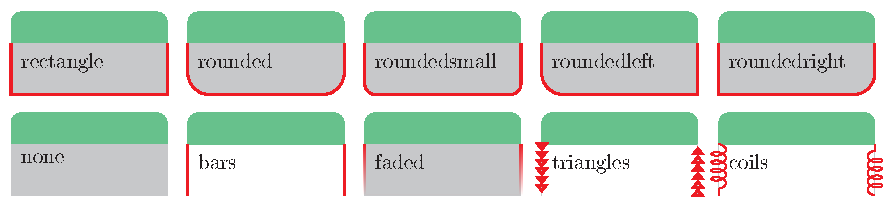
\includegraphics[width=.8\textwidth, ]{docs-boxshape}}
    \item \lr{\texttt{headerborder=header border type}}:
    آن بخشی از جعبه که پیرامون عنوان قرار می گیرد را تعیین می‌کند:

    \centerline{
\includegraphics[width=.8\textwidth, ]{docs-headerborder}}
    \item \lr{\texttt{headershape=header border shape}}:
    نوع آرایش عنوان جعبه را مشخص می‌کند:

    \centerline{
\includegraphics[width=.8\textwidth, ]{docs-headershape}}
    \item \lr{\texttt{headershade=type of header shading}}:

%        \begin{enumerate*}[label=\arabic*)]
%            \item\texttt{plain}
%            \item\texttt{shadelr}
%            \item\texttt{shaderl}
%            \item\texttt{shadetb}
%            \item\texttt{shadetbinverse}
%        \end{enumerate*}

    \centerline{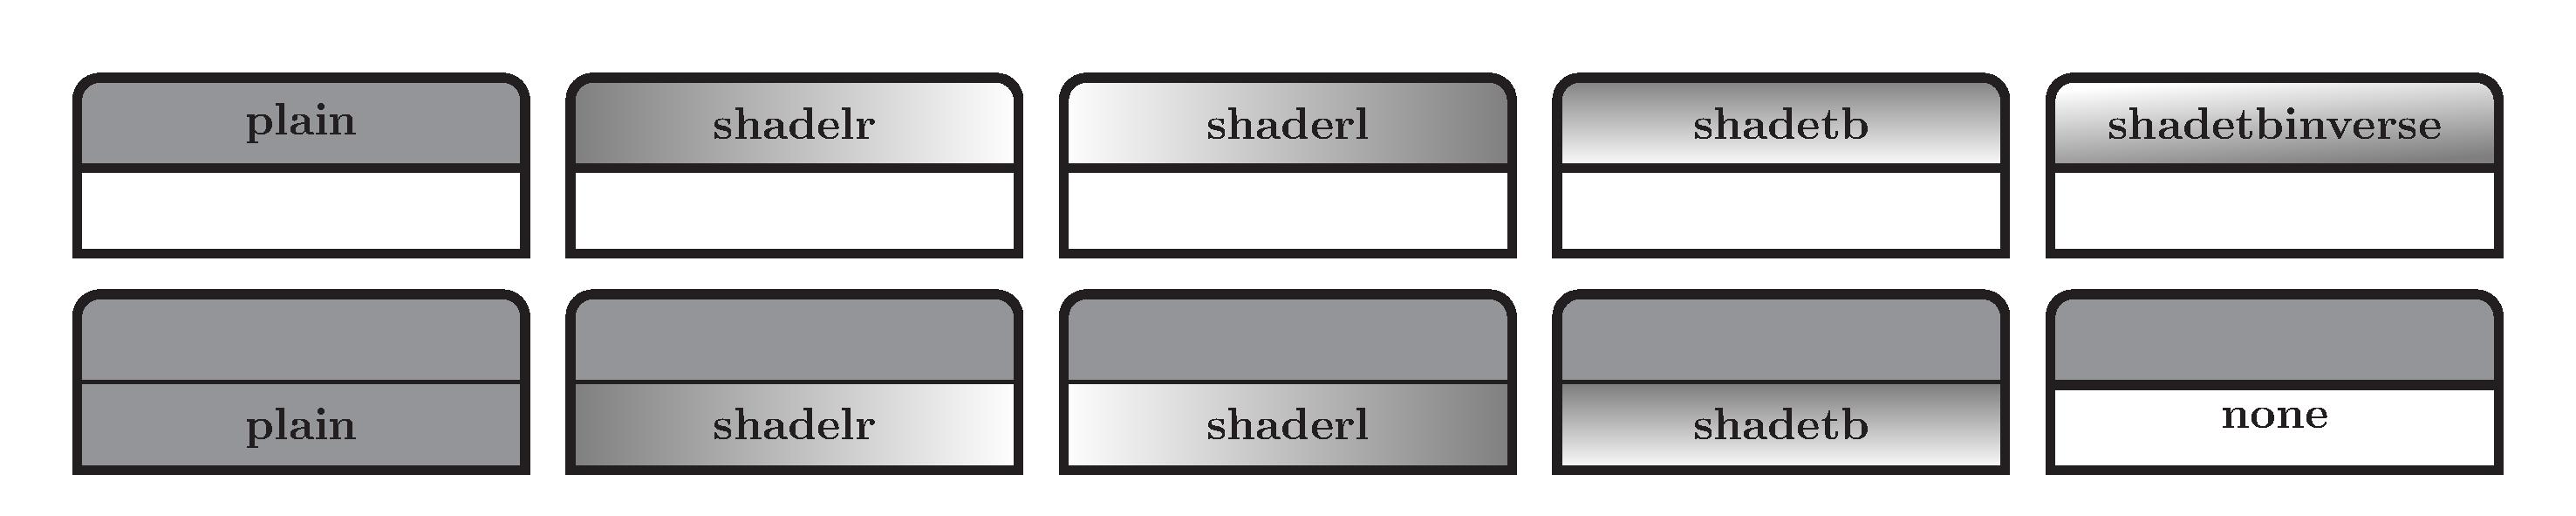
\includegraphics[width=.82\textwidth,
    trim={.4cm 5.1cm .4cm .6cm}, clip=true]{docs-shade.pdf}}

    \item \lr{\texttt{boxshade}}:

%        \begin{enumerate*}[label=\arabic*)]
%            \item\texttt{plain}
%            \item\texttt{shadelr}
%            \item\texttt{shaderl}
%            \item\texttt{shadetb}
%            \item\texttt{none}
%        \end{enumerate*}

    \centerline{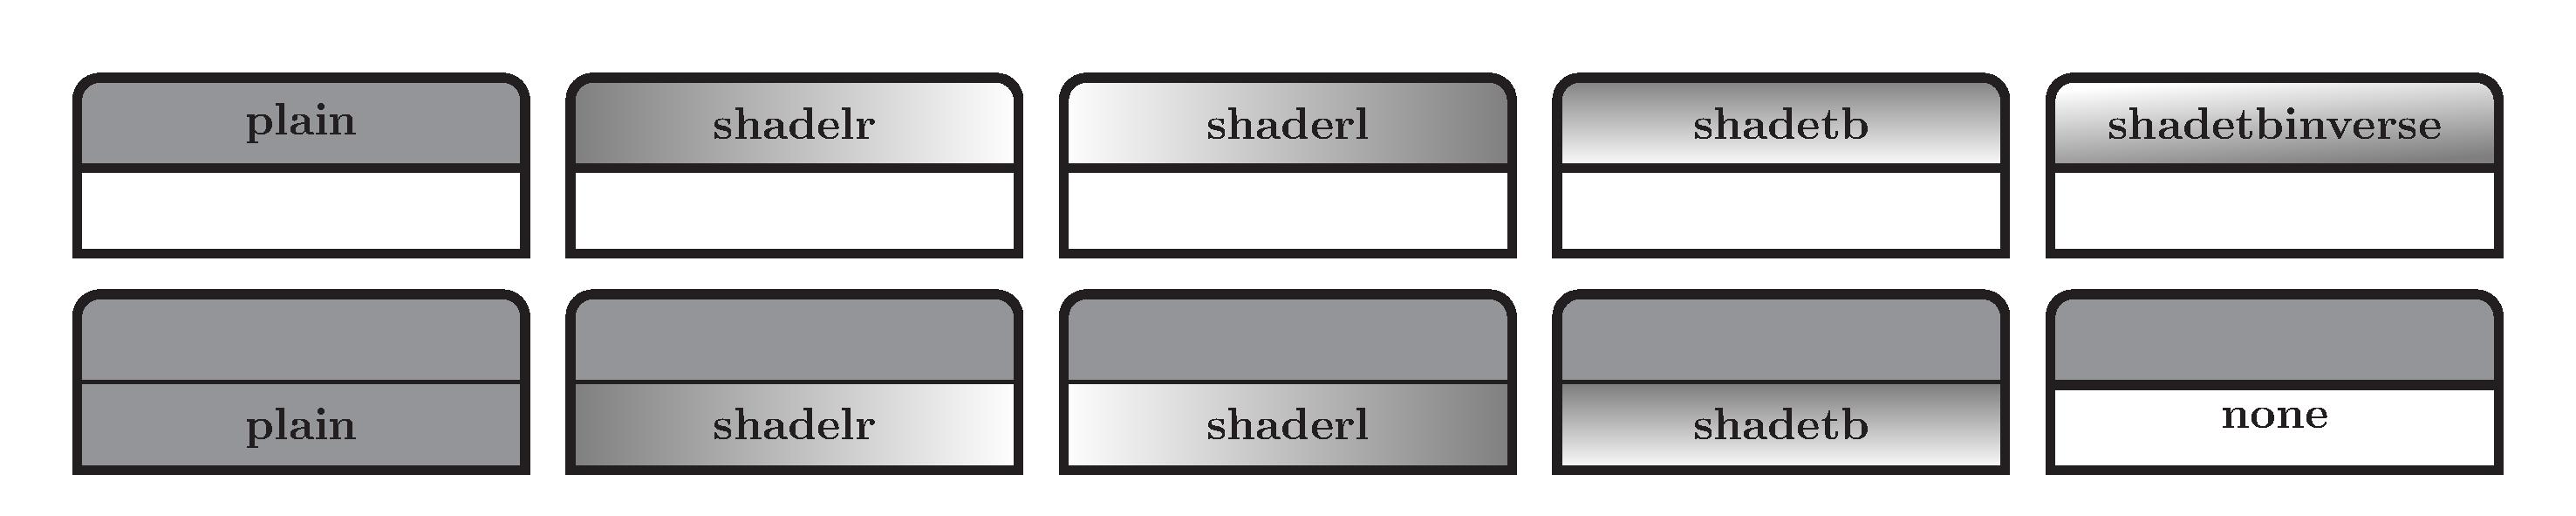
\includegraphics[width=.82\textwidth,
    trim={.4cm .1cm .4cm 5.5cm}, clip=true]{docs-shade.pdf}}

    \item \lr{\texttt{headerfont=font definition}}:
    دستوری که قبل از حروفچینی عنوان جعبه قرار داده می‌شود.
    \item \lr{\texttt{headerFontColor=pgf color name}}:
    رنگ قلم عنوان جعبه.
    \item \lr{\texttt{linewidth=length}}:
    عرض خطوط مورد استفاده در ترسیم پوستر
    \item \lr{\Verb|above=box name|}:
    نام جعبه‌ای را مشخص می‌کند که این جعبه باید در بالای جعبه مذکور ترازبندی شود.
    \item \lr{\Verb|below=box name|}:
    نام جعبه‌ای را مشخص می‌کند که این جعبه باید در پایین جعبه مذکور ترازبندی شود.
    \item \lr{\Verb|aligned=box name|}:
    نام جعبه‌ای را مشخص می‌کند که این جعبه باید به محاذات آن جعبه ترازبندی شود.
    \item \lr{\Verb|bottomaligned=box name|}:
    نام جعبه‌ای را مشخص می‌کند که این جعبه باید نسبت به آن جعبه از پایین ترازبندی شود.
\end{itemize}
\end{posterbox}
 %%%%%%%%%%%%%%%%%%%%%%%%%%%%%%%%%%%%%%%%%%%%%%%%%%%%%%%%%%%%%%%%%%%%%%%%%%%%%%
\begin{posterbox}[name=absolute,column=0,span=2,below=setting,
,textborder=rectangle,headershape=rectangle,]{چینش جعبه‌ها}
%\small
    نکته‌ای که باید در چینش جعبه‌ها در نظر داشته باشید این است که مکان جعبه‌ها می‌توانند به صورت نسبی یا دقیق تعیین شود.
    اگر برای مثال جعبه ب قرار است دقیقاً بین جعبه‌های الف و ج قرار گیرد
    آنگاه این دو جعبه اخیر حتماً باید پیش از جعبه ب تعریف شوند، در غیر اینصورت سبب تولید خطا می‌گردد. ضمناً می‌توانید بدون
    تعیین این پارامترها چینش جعبه‌ها را به صورت خودکار و بهمان ترتیب تعریف به خود بسته واگذار نمایید.

    برای آدرس‌دهی دقیق یک جعبه، جایگاه دقیق آن‌ را با کمک \Verb|row| و \Verb|column|
    در تنظیمات جعبه‌پوستر مشخص نمایید.
\end{posterbox}
 %%%%%%%%%%%%%%%%%%%%%%%%%%%%%%%%%%%%%%%%%%%%%%%%%%%%%%%%%%%%%%%%%%%%%%%%%%%%%%
\begin{posterbox}[name=ack,column=3,span=2,below=posterboxoption, bottomaligned=absolute,
,textborder=triangles]{قدردانی}
 %%%%%%%%%%%%%%%%%%%%%%%%%%%%%%%%%%%%%%%%%%%%%%%%%%%%%%%%%%%%%%%%%%%%%%%%%%%%%%
با تشکر از دکتر \lr{Brian} خالق کلاس پوستر و تشکر ویژه از جناب آقای دکتر وفا خلیقی بخاطر زحماتی که برای فارسی‌نویسی در
محیط زی‌لاتک انجام‌ داده‌اند %\footnote{بدون پشتیبانی زی‌پرشین از محیط \lr{tikzpicture} فارسی سازی این کلاس ممکن نبود.}
 و دکتر محمود امین‌طوسی به سبب پیشنهاد نام زیباپوستر و گروه پارسی‌لاتک برای تست این کلاس.

\footnotetext{
زیباپوستر از نسخهٔ $2.2$ به بعد بر خلاف نسخه اولیّه هر دو نوع پوستر پارسی و لاتین را پشتیبانی می‌کند. }
\end{posterbox}
%%%%%%%%%%%%%%%%%%%%%%%%%%%%%%%%%%%%%%%%%%%%%%%%%%%%%%%%%%%%%%%%%%%%%%%%%%%%%%
\end{poster}
\end{document}
